\begin{question}
\noindent Triangle $A$ has vertices at $(1,1)$, $(1,3)$ and $(3,1)$.

Triangle $B$ has vertices at $(1,-1)$, $(3,-1)$ and $(1,-3)$.

Triangle $B$ is the image of triangle $A$ after a single transformation.

\begin{center}
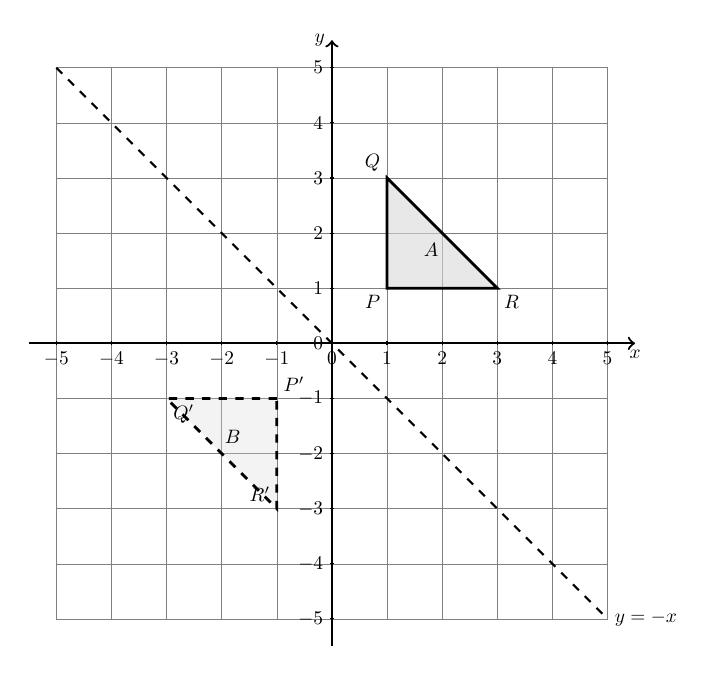
\begin{tikzpicture}[scale=0.7, transform shape]
    % Define colours
    \definecolor{borderColour}{HTML}{000000}
    \definecolor{fillColour}{HTML}{D8D8D8}

    % Define axis scale
    \def\axisLimit{5}

    % Draw grid
    \draw[step=1cm,gray,very thin] (-\axisLimit,-\axisLimit) grid (\axisLimit,\axisLimit);

    % Draw axes
    \draw[thick,->] (-\axisLimit-0.5,0) -- (\axisLimit+0.5,0) node[anchor=north] {$x$};
    \draw[thick,->] (0,-\axisLimit-0.5) -- (0,\axisLimit+0.5) node[anchor=east] {$y$};

    % Label x-axis and y-axis
    \foreach \x in {-\axisLimit,...,\axisLimit}
        \draw (\x cm,1pt) -- (\x cm,-1pt) node[anchor=north] {$\x$};
    \foreach \y in {-\axisLimit,...,\axisLimit}
        \draw (1pt,\y cm) -- (-1pt,\y cm) node[anchor=east] {$\y$};

    % Draw the mirror line y = -x
    \draw[thick,dashed] (-5,5) -- (5,-5) node[anchor=west] {$y=-x$};

    % Define coordinates for triangle A
    \coordinate (P) at (1,1);
    \coordinate (Q) at (1,3);
    \coordinate (R) at (3,1);

    % Draw triangle A
    \filldraw[fill=fillColour, draw=borderColour, line width=1pt, fill opacity=0.6] (P) -- (Q) -- (R) -- cycle;

    \node[below left] at (P) {$P$};
    \node[above left] at (Q) {$Q$};
    \node[below right] at (R) {$R$};
    \node at (1.8,1.7) {$A$};

    % Define coordinates for triangle B
    \coordinate (P') at (-1,-1);
    \coordinate (Q') at (-3,-1);
    \coordinate (R') at (-1,-3);

    % Draw triangle B
    \filldraw[fill=fillColour, draw=borderColour, line width=1pt, fill opacity=0.3, dashed] (P') -- (Q') -- (R') -- cycle;

    \node[above right] at (P') {$P'$};
    \node[below right] at (Q') {$Q'$};
    \node[above left] at (R') {$R'$};
    \node at (-1.8,-1.7) {$B$};

\end{tikzpicture}
\end{center}

\noindent Describe fully the single transformation that maps triangle $A$ onto triangle $B$.

\vspace{4cm}
\answerlines{3}{3}
\end{question}